\section*{Введение}
\addcontentsline{toc}{section}{Введение}
	\subsection*{Актуальность проблемы}
	\addcontentsline{toc}{subsection}{Актуальность проблемы}
		\hspace{1em} 	Задача очищения атмосферного воздуха от загрязняющих выбросов промышленных предприятий достаточно актуальна. Выбросы от стационарных источников вредных веществ в атмосферу городов и населенных пунктов, расположенных на территории северо-западного федерального округа,  по данным Росстата за 2007 год,  составили 2319000 тонн, в том числе твёрдых -- 289400 тонн \cite{emissionInfoRussian}. В некоторых отраслях промышленности доля выбросов пыли в атмосферу достигает 15\% от общего числа получаемого продукта. Так, при изготовлении одной тонны цемента в воздух выбрасывается $\approx 160$ кг цементной пыли \cite{emissionInfoEurope}.
		\begin{figure}[ht]
			\begin{minipage}{0.46\linewidth}
				\vspace{-1em}
				Динамика изменения объёма выбросов твёрдых вредных веществ в атмосферу \textit{(рисунок \ref{figure:atmosphereDynamic})} имеет тенденцию к росту, что говорит о том, что решение проблемы инженерной защиты воздуха от вредных веществ останется актуальной и в ближайшем будущем. 
			\end{minipage}
			\hspace{0.01\linewidth}
			\begin{minipage}{0.48\linewidth}
				\centering
				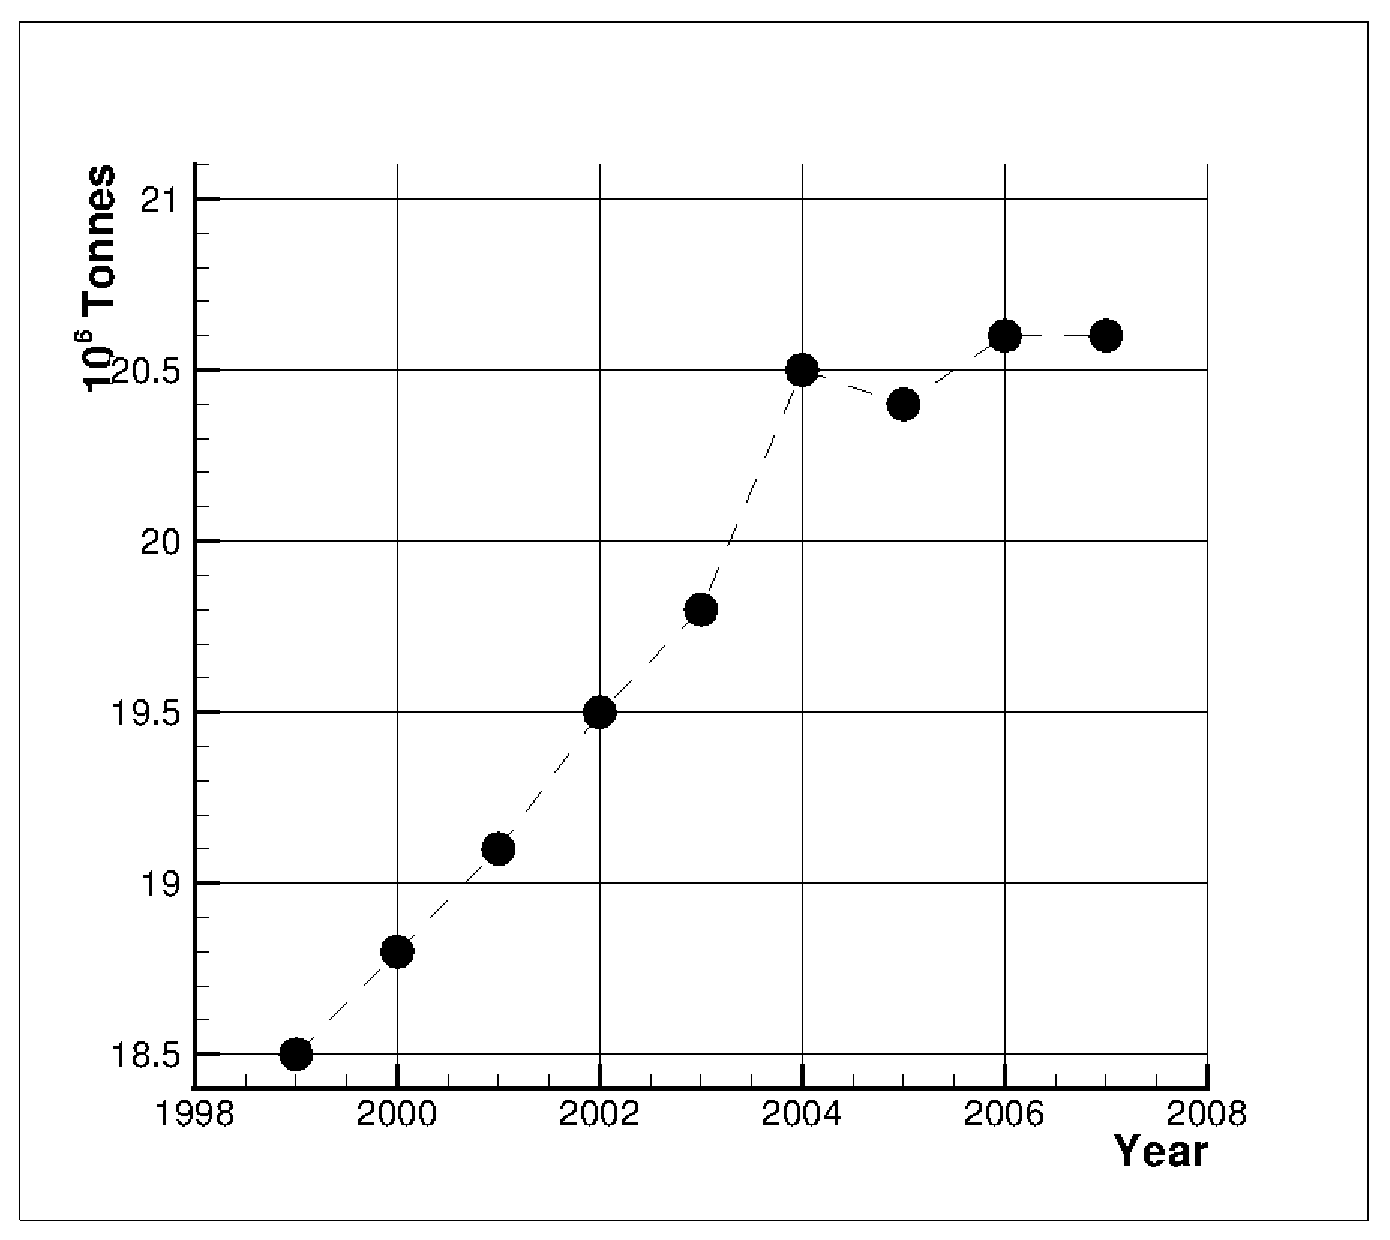
\includegraphics[scale=0.26]{atmosphereDynamic1}
				\caption{Динамика выбросов твёрдых веществ в атмосферу \cite{emissionInfoRussian}}
				\label{figure:atmosphereDynamic}
			\end{minipage}
		\end{figure}
		\vspace{-1em}
	
		Для очищения воздуха от твёрдых примесей широкое распространение получили фильтры типа циклон. Циклон представляет собой инерционный пылеуловитель, в котором выделение частиц из воздушной среды происходит, в основном, под действием центробежной силы, возникающей при вращении воздушного потока в корпусе аппарата.
	
		Запылённый воздух входит в циклон через тангенциальный патрубок и, приобретая вращательное движение, опускается винтообразно вниз вдоль внутренних стенок цилиндра и конуса. Небольшая часть этого потока, в котором сконцентрированы пылевые частицы, движется в непосредственной близости от стенок циклона и поступает через пылеотводящее отверстие в пылесборный бункер, где происходит осаждение и накопление пылевых частиц.
	
		В центральной зоне циклона воздушный поток, освобождённый от пыли, поднимается винтообразно вверх и удаляется через выхлопную трубу наружу.
	
		Вследствие вращательного движения воздушного потока в центральной зоне циклона (в конусе, выхлопной трубе и пылесборном бункере) наблюдается пониженное давление.\cite{instructions}
	
		В силу высокой степени закрученности потока, необходимо введение поправок в модели турбулентности для учёта кривизны линий тока. Кроме того, учитывая высокую концентрацию частиц в потоке, в инженерных расчётах необходимо учитывать не только влияние потока на частицы, но также и обратное влияние частиц на поток.
	%Актуальность проблемы
	\subsection*{Цели работы}
	\addcontentsline{toc}{subsection}{Цели работы}
		\begin{enumerate}
			\item Реализация $k-\omega-SST$ модели турбулентности с поправкой на кривизну линий тока при помощи открытой интегрируемой платформы для численного моделирования задач механики сплошных сред OpenFOAM.
			\item Реализация с использованием OpenFOAM солвера, имеющего в основе модель идеального газа и учитывающего при этом обратное влияние частиц на поток.
			\item Численное моделирование циклона с учётом обратного влияния частиц на поток и поправки на кривизну линий тока к генерации турбулентности.
		\end{enumerate}
	%Цели работы
%Введение
